\documentclass[a4paper, 12pt, twoside]{article}
\usepackage[utf8]{inputenc}		% LaTeX, comprend les accents !
\usepackage[T1]{fontenc}		
\usepackage[francais]{babel}
\usepackage{lmodern}
\usepackage{ae,aecompl}
\usepackage[top=2.5cm, bottom=2cm,
			left=3cm, right=2.5cm,
			headheight=15pt]{geometry}
\usepackage{graphicx}
\usepackage{eso-pic}	% Nécessaire pour mettre des images en arrière plan
\usepackage{array} 
\usepackage{hyperref}
%%%%%%%%%%%%%%%%%%%%%%%%%%%%%%%%%%%%%%%%
%    Page de garde (Pagedegarde.tex)   %
%%%%%%%%%%%%%%%%%%%%%%%%%%%%%%%%%%%%%%%%
% Dorian Depriester, 2014

\makeatletter
\def\@ecole{école}
\newcommand{\ecole}[1]{
  \def\@ecole{#1}
}

\def\@entreprise{Nom de l'entreprise}
\newcommand{\entreprise}[1]{
  \def\@entreprise{#1}
}

\def\@datedebut{\today}
\newcommand{\datedebut}[1]{
  \def\@datedebut{#1}
}


\def\@github{}
\newcommand{\github}[1]{
  \def\@github{#1}
}

\def\@datefin{\today}
\newcommand{\datefin}[1]{
  \def\@datefin{#1}
}



\def\@specialite{Spécialité}
\newcommand{\specialite}[1]{
  \def\@specialite{#1}
}

\def\@ED{\'{E}cole Doctorale}
\newcommand{\ED}[1]{
  \def\@ED{#1}
}

\def\@doctorat{Doctorat}
\newcommand{\doctorat}[1]{
  \def\@doctorat{#1}
}

\def\@adresse{Adresse}
\newcommand{\adresse}[1]{
  \def\@adresse{#1}
}

\def\@directeur{directeur}
\newcommand{\directeur}[1]{
  \def\@directeur{#1}
}

\def\@encadrant{encadrant}
\newcommand{\encadrant}[1]{
  \def\@encadrant{#1}
}
\def\@membrea{Membre}
\newcommand{\membrea}[1]{
  \def\@membrea{#1\\}
}
\def\@membreb{Membre}
\newcommand{\membreb}[1]{
  \def\@membreb{#1\\}
}
\def\@membrec{Membre}
\newcommand{\membrec}[1]{
  \def\@membrec{#1\\}
}






\def\@juryb{}{}{}
\newcommand{\juryb}[3]{
  \def\@juryb{#1,	& #2	& #3\\}
}
\def\@juryc{}{}{}
\newcommand{\juryc}[3]{
  \def\@juryc{#1,	& #2	& #3\\}
}
\def\@juryd{}{}{}
\newcommand{\juryd}[3]{
  \def\@juryd{#1,	& #2	& #3\\}
}
\def\@jurye{}{}{}
\newcommand{\jurye}[3]{
  \def\@jurye{#1,	& #2	& #3\\}
}
\def\@juryf{}{}{}
\newcommand{\juryf}[3]{
  \def\@juryf{#1,	& #2	& #3\\}
}
\def\@juryg{}{}{}
\newcommand{\juryg}[3]{
  \def\@juryg{#1,	& #2	& #3\\}
}
\def\@juryh{}{}{}
\newcommand{\juryh}[3]{
  \def\@juryh{#1,	& #2	& #3\\}
}
\def\@juryi{}{}{}
\newcommand{\juryi}[3]{
  \def\@juryi{#1,	& #2	& #3\\}
}
\makeatother

\newcommand\BackgroundPic{%
	\put(0,0){%
		\parbox[b][\paperheight]{\paperwidth}{%
			\includegraphics[height=0.45\paperheight]{bordure.png}%
			\vfill
		}
	}
}
\newcommand\EtiquetteThese{%
	\put(0,0){%
		\parbox[t][\paperheight]{\paperwidth}{%
			\hfill
			%\colorbox{blue}{		
				\begin{minipage}[b]{2em}
					\includegraphics[width=4.0\textwidth]{logo_miage.png}\\					
					%\centering\Huge\textcolor{white}{M\\I\\A\\G\\E\\}
					\vspace{0.2cm}
				\end{minipage}
			%}
		}
	}
}

\makeatletter
\newcommand{\pagedegarde}{
\newgeometry{top=2.5cm, bottom=1cm, left=2cm, right=1cm}
\AddToShipoutPicture*{\BackgroundPic}
%\AddToShipoutPicture*{\EtiquetteThese}
  \begin{titlepage}
  \centering
      
\includegraphics[width=0.6\textwidth]{logo_Paris_Nanterre_couleur_RVB.png}
      \hfill
      $\ $\\
      %\includegraphics[width=0.20\textwidth]{logo_entreprise.png}\\
    \vspace{1cm}
      {\Large Licence MIASHS première année}\\
    \vspace{1cm}
      {\huge 
      	{\bfseries Rapport de projet informatique}\\
    \vspace{0.5cm}}
      	$\ $\\
    \vspace{1cm}
   		
    \vspace{1cm}
    	{\huge\color[rgb]{0,0,1} \bfseries{\@title}}\\
    \vspace{0.5cm}
    %{\bfseries Entreprise d'accueil : \@entreprise}\\
    {\bfseries Projet réalisé du \@datedebut\ au \@datefin}\\
    %	{\Large{\bfseries Spécialité doctorale ``\@specialite''}}\\
    \vspace{2cm}
    $\ $\\
    \vspace{0.5cm}
    $\ $\\
    \vspace{0.5cm}
    %	le \@date \\
    \vfill
     %  {\LARGE \color[rgb]{0,0,1} \bfseries{\@title}} \\
    %\vfill
      %  Directeur de thèse : {\bfseries \@directeur}\\
       % Co-encadrant de thèse : {\bfseries \@encadrant}\\
    %\vfill
    \textbf{Lien GitHub du projet :} \url{https://github.com/YahyaA86/Plateforme-de-codage-} \\[1cm]
	\begin{tabular}{>{\bfseries}lll}
		\large Membres du groupe\\
		\vspace{0.15cm}\\
		\@membrea
		\@membreb
		\@membrec
		\@membred
		\@membree
		%\@jurye
		%\@juryf
		%\@juryg
		%\@juryh
		%\@juryi
	\end{tabular}
	%\includegraphics[width=0.20\textwidth]{logo_entreprise.png}\
	\vfill
	
	%\@adresse
  \end{titlepage}




\restoregeometry  
}



\title{Plateforme de génération d'exercices de programmation corrigés automatiquement par une IA}
\entreprise{Projet académique - Plateforme Ollama}
\datedebut{15 avril 2025}
\datefin{30 avril 2025}
\ecole{Université Paris Nanterre, Département d'Informatique}



\membrea{YAHYA AKIL 44005696}
\membreb{MEHDI BELABBAS 44000690}
\membrec{KARIM ABDALLAH 44020626}


\begin{document}

\pagestyle{empty}
\pagedegarde
\newpage

\tableofcontents
\newpage

\section{Introduction}

Ce rapport présente la conception et le développement d'une plateforme web de génération d'exercices de programmation corrigés automatiquement par une intelligence artificielle. La plateforme vise à aider les débutants en codage en proposant des exercices adaptés aux langages et aux thèmes choisis par l'utilisateur. Elle permet de gagner du temps en générant dynamiquement du contenu pédagogique (énoncés d'exercice, exemples de solution, sorties attendues) sans intervention manuelle. Le point central du projet est l'utilisation d'un modèle de langage avancé, via Ollama, pour créer et corriger les exercices. Nous allons détailler dans ce rapport les fonctionnalités implémentées, l'architecture utilisée, ainsi que les défis techniques rencontrés au cours du développement.

\begin{figure}[h!]
\centering
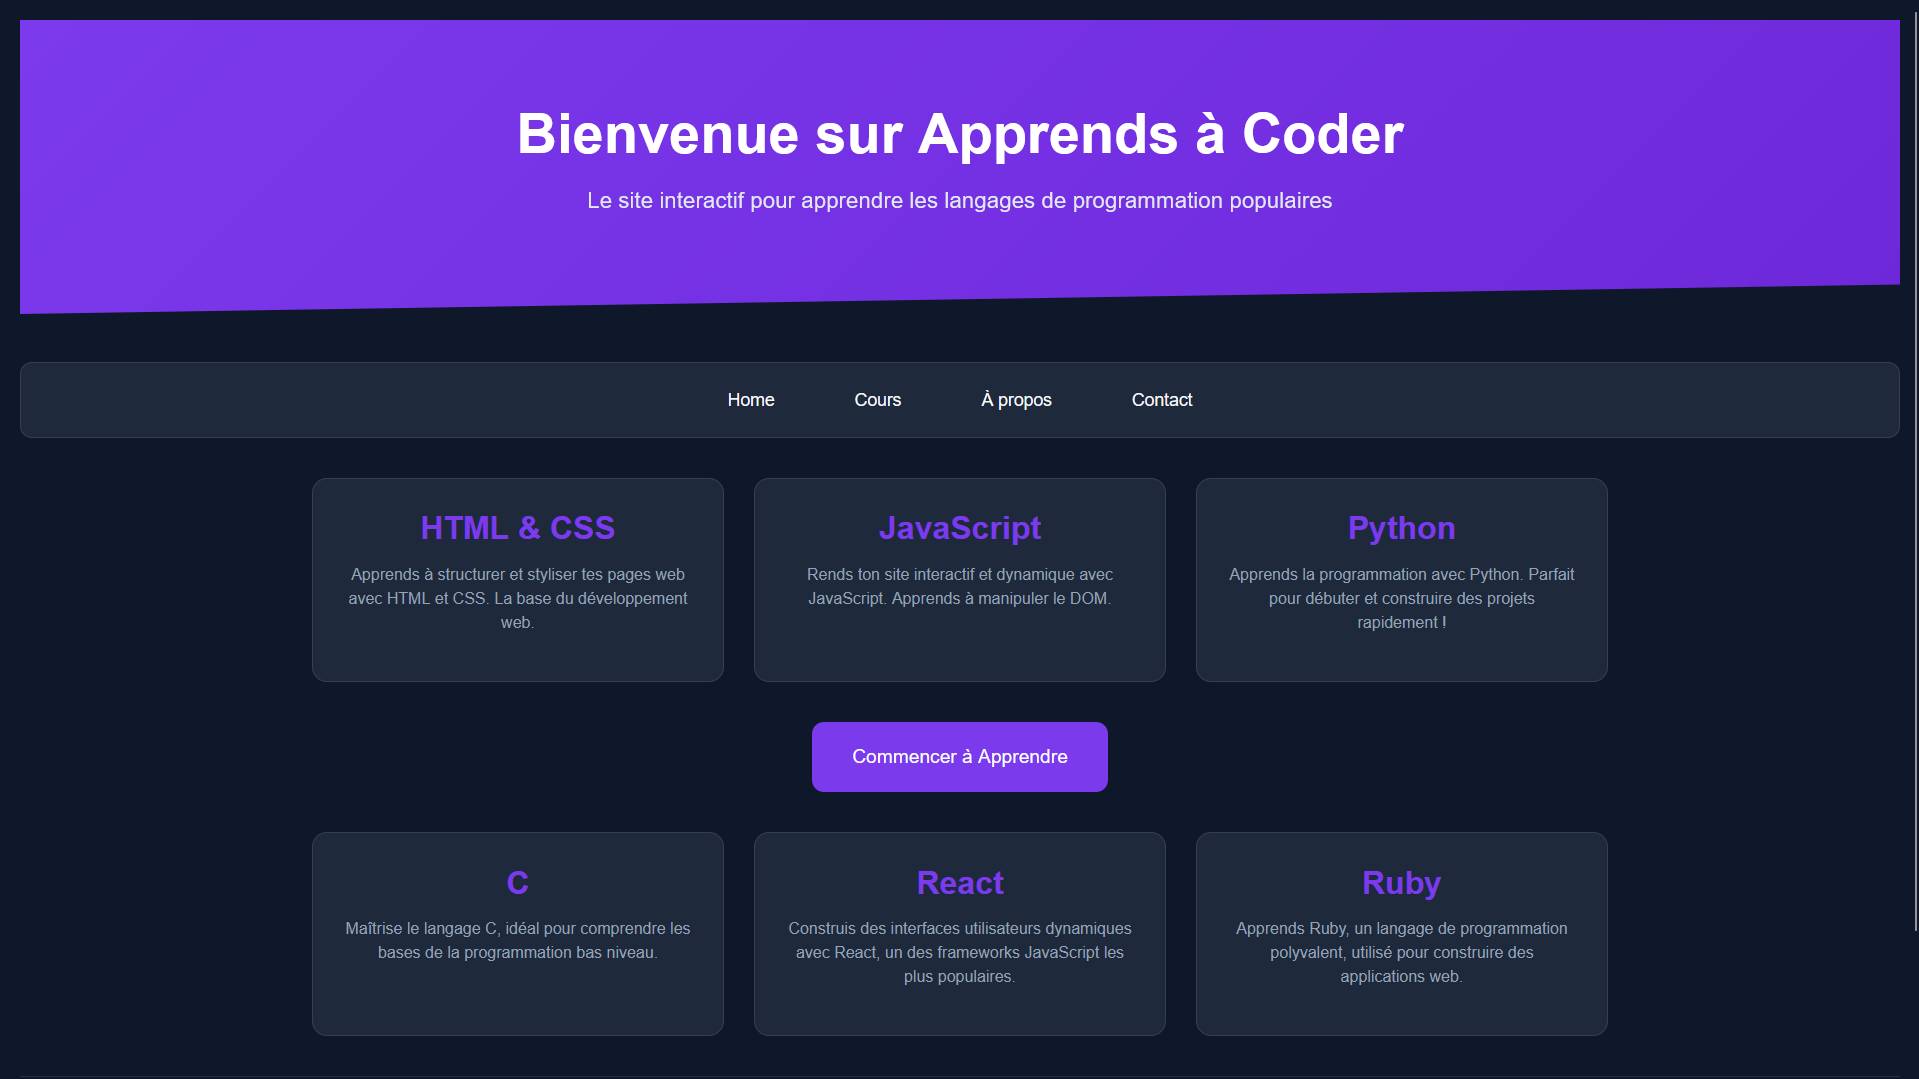
\includegraphics[width=1.2\textwidth]{pageaccueil.png}
\caption{Page d'accueil de la plateforme (interface principale).}
\label{fig:pageaccueil}
\end{figure}

\section{Environnement de travail}

L'application a été développée en Python 3 avec le framework Flask pour le backend, et utilise HTML/CSS/JavaScript pour le frontend. Nous avons installé Ollama sur la machine pour accéder au modèle de langage (Mistral) localement via une API Python. Pour exécuter et tester les exercices de code, l'environnement inclut des compilateurs ou interpréteurs pour les langages supportés (Python, JavaScript, C, Java, Ruby), comme l'illustre le serveur configuré avec les commandes d'exécution correspondantes. L’interface a été testée sous différents navigateurs récents pour garantir la compatibilité, et le projet a été développé sous Windows, tout en étant également vérifié sous Linux afin d’assurer une compatibilité multiplateforme. 

\section{Description du projet et objectifs}

Ce projet consiste en une plateforme web qui permet à l'utilisateur de générer automatiquement des exercices de programmation corrigés. L'utilisateur choisit un thème (par exemple, un concept de programmation) et un langage (Python, Java, JavaScript, C, Ruby) via un formulaire dédié. En cliquant sur le bouton de génération, la plateforme envoie ces paramètres à l'IA pour créer un nouvel exercice. L'exercice généré comprend un énoncé détaillé, des consignes claires, ainsi qu'une solution commentée encadrée par un bloc de code, accompagnée de la sortie attendue. Par la suite, l'utilisateur peut modifier le code de l'exercice ou écrire sa propre solution et utiliser l'éditeur intégré pour l'exécuter et vérifier les résultats. Les principaux objectifs du projet sont de fournir un outil interactif d'apprentissage du code, d'automatiser la création de contenu pédagogique, et de se familiariser avec l'utilisation d'API d'IA moderne.

\section{Bibliothèques, Outils et technologies}

La plateforme repose sur plusieurs technologies : le backend utilise Flask en Python, ainsi que la bibliothèque Ollama pour interagir avec l'intelligence artificielle. Pour le frontend, nous utilisons HTML5, CSS3 et JavaScript pour créer une interface utilisateur réactive. Le traitement du texte Markdown est assuré par la bibliothèque Python \texttt{markdown} pour formater l'exercice et la réponse de l'IA en HTML affiché sur la page. Le code Python pour l'exécution d'exercices de différents langages repose sur les commandes systèmes (via \texttt{subprocess}) associées aux interpréteurs ou compilateurs installés. Enfin, l'API Flask et les requêtes AJAX en JavaScript assurent la communication entre le frontend et le serveur.

\section{Travail réalisé}

Dans la partie ``Travail réalisé'', nous décrivons la mise en œuvre des principales fonctionnalités. Le point de départ est l'interface utilisateur qui permet de paramétrer un exercice. 

\begin{figure}[h!]
\centering
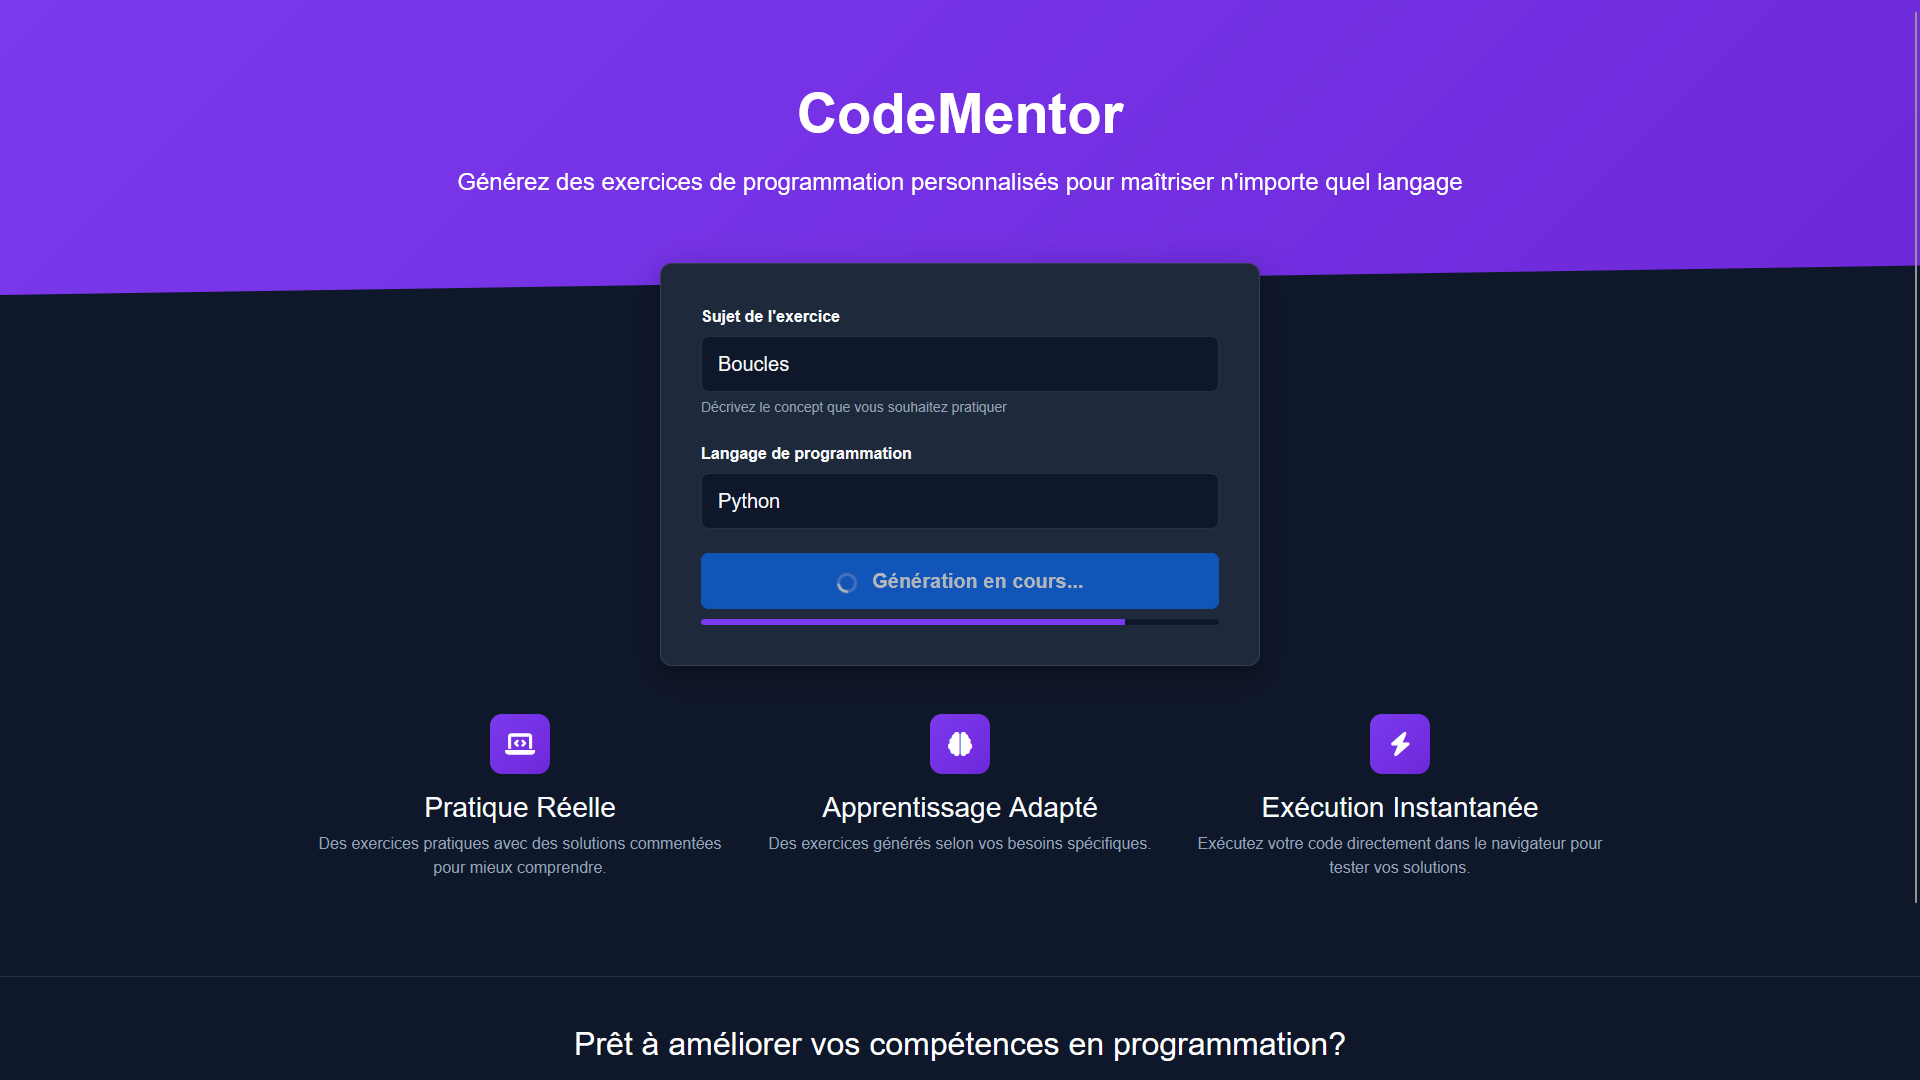
\includegraphics[width=1.2\textwidth]{formulaire.png}
\caption{Interface du formulaire de génération d'exercice.}
\label{fig:formulaire}
\end{figure}

Lorsque l'utilisateur soumet le formulaire, une requête AJAX envoie le thème et le langage choisis au serveur Flask. Le serveur appelle alors la fonction de génération qui construit un prompt destiné à l'IA Ollama. Par exemple, le prompt inclut un texte demandant de créer un exercice complet en spécifiant le langage et le thème. Voici un extrait de prompt envoyé au modèle : 

\begin{verbatim}
Crée un exercice de programmation complet en Python sur le thème: boucles. Fournis une description claire, des consignes précises, un exemple de solution bien commenté entre triple backticks avec le label 'Solution', et la sortie attendue. Formatte le tout en markdown.
\end{verbatim}

La réponse de l'IA est reçue au format texte Markdown. Nous utilisons une expression régulière pour extraire le code de la solution encadré par \texttt{```} et séparer l'énoncé de l'exercice. Le code de la solution est ensuite stocké et affiché dans l'éditeur de l'interface utilisateur. Il est à noter que chaque exercice généré est également mis en cache pour éviter des appels redondants à l'IA lors d'une demande identique.

\section{Difficultés rencontrées}

Plusieurs difficultés ont été rencontrées lors du développement. L'une des principales était la manipulation du contenu Markdown renvoyé par l'IA : il a fallu nettoyer le texte pour extraire correctement la partie exercice et la solution encadrée par les balises \texttt{```} en utilisant des expressions régulières. Nous avons également dû gérer l'encodage Unicode (pour les accents ou caractères spéciaux) afin d'éviter des erreurs lors du traitement du texte. Parfois l'API Ollama mettait du temps à répondre ou retournait des erreurs de temps d'exécution, ce qui a nécessité l'implémentation de délais (timeouts) et la gestion d'exceptions pour informer l'utilisateur en cas de problème. Sur le plan frontend, intégrer les requêtes AJAX avec Flask a nécessité d'activer CORS et de formater correctement les données JSON échangées. Enfin, nous avons dû gérer l'exécution des différents langages de programmation en veillant à nettoyer les fichiers temporaires et à gérer les erreurs de compilation ou d'exécution renvoyées par l'interpréteur. Chaque obstacle a été surmonté par une recherche de solutions adaptées (ajustement des expressions régulières, gestion des erreurs \texttt{try/except} en Python, etc.), améliorant ainsi la robustesse de la plateforme.

\section{Bilan}

En conclusion, ce projet nous a permis de mettre en pratique plusieurs compétences techniques. L'utilisation de LaTeX pour rédiger ce rapport a été l'occasion d'apprendre la structuration de documents et l'inclusion d'éléments tels que des images et des figures. L'intégration de l'IA Ollama dans une application web nous a familiarisés avec les API de modèles de langage et la conception de prompts efficaces. Le développement du backend Flask et du frontend dynamique a renforcé nos connaissances en programmation web (gestion des requêtes, traitement des réponses JSON, mise en page HTML/CSS/JavaScript). Le projet a aussi permis de travailler sur la gestion des erreurs et le débogage de bout en bout : capturer et traiter les exceptions (dans les appels à l'IA, à l'exécution du code), et sécuriser les échanges de données. Enfin, la génération dynamique de contenu pédagogique nous a appris à concevoir des algorithmes réactifs et à orchestrer plusieurs composants logiciels pour répondre à une demande utilisateur.

\section{Bibliographie}
\renewcommand{\bibname}{}
\renewcommand{\refname}{}
\begin{thebibliography}{2}
\bibitem[label]{cle} Auteur, TITRE, éditeur, année
\bibitem[LAM94]{lam1} L. LAMPORT, {\it \LaTeX: A Document Preparation System}, Addison-Wesley, 1994.
\end{thebibliography}

\newpage
\section{Webographie}
\begin{thebibliography}{2}
\bibitem[CAT]{cat} \url{savoircoder.fr/cat}
\bibitem[Flask]{flask} \url{https://flask.palletsprojects.com/}
\bibitem[Python]{python} \url{https://docs.python.org/}
\bibitem[Ollama]{ollama} \url{https://ollama.readthedocs.io/en/quickstart/}
\bibitem[HTML]{html} \url{https://developer.mozilla.org/fr/docs/Web/HTML}
\end{thebibliography}

\newpage
\section{Annexes}
\appendix
\makeatletter
\def\@seccntformat#1{Annexe~\csname the#1\endcsname:\quad}
\makeatother

	\section{Cahier des charges}
Ce cahier des charges précisait les fonctionnalités attendues du projet : La plateforme doit permettre la génération d'exercices personnalisés en fonction du thème et du langage choisis, afficher l'énoncé et la solution du chatbot, et exécuter le code fourni. L'interface utilisateur simple doit être accessible via un navigateur web et communiquer avec un backend prenant en charge l'IA Ollama. Les exigences techniques incluaient l'utilisation de Flask pour le serveur, l'intégration d'Ollama pour la génération de texte, et la capacité d'exécuter du code dans plusieurs langages de programmation.

	\section{Exemple d'exécution du projet}
L'annexe présente un exemple concret d'exercice généré automatiquement par la plateforme, avec sa solution associée. 

\begin{figure}[h!]
\centering
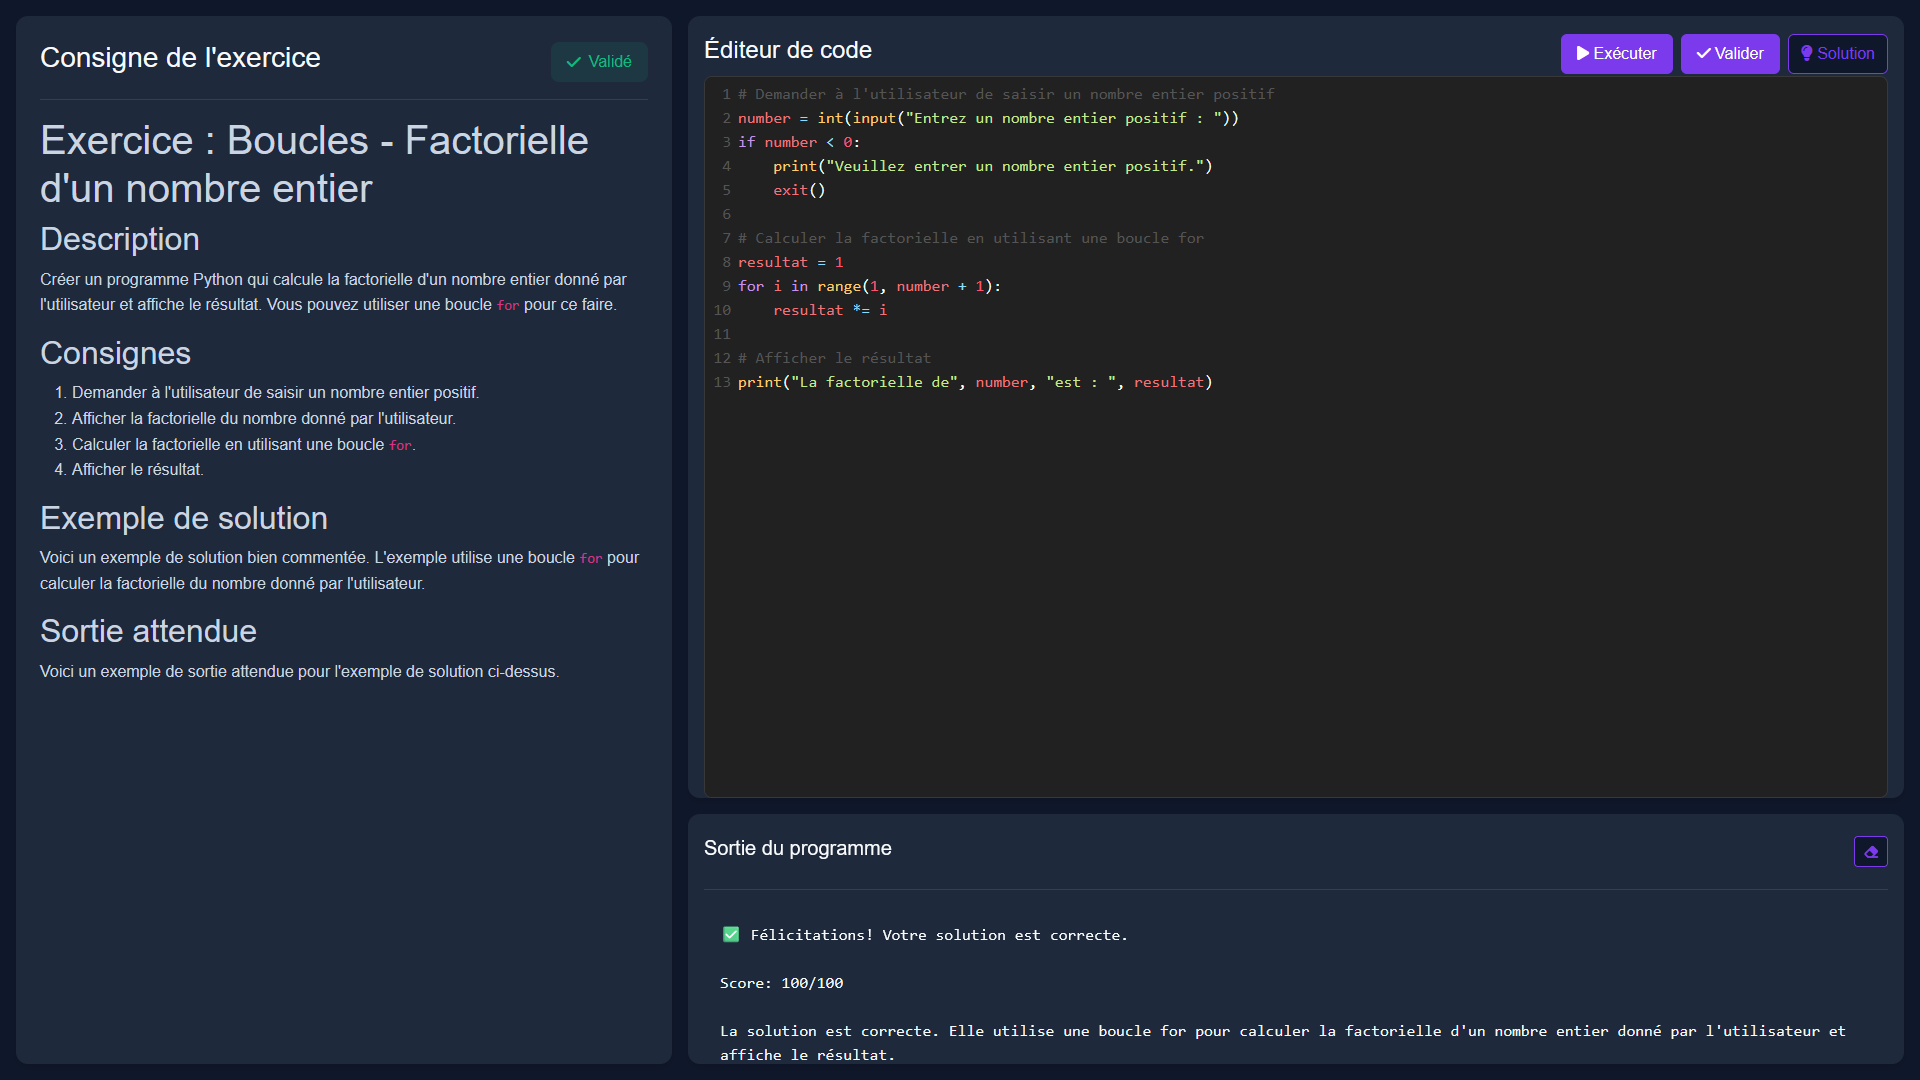
\includegraphics[width=1.3\textwidth]{exercice.png}
\caption{Exemple d'exercice généré par l'IA, avec sa solution.}
\label{fig:exercice}
\end{figure}

	\section{Manuel utilisateur}
Le manuel utilisateur décrit l'utilisation de la plateforme : après avoir lancé le serveur Flask avec \texttt{python app.py}, l'utilisateur accède à l'application via son navigateur à l'adresse locale : \texttt{http://localhost:5000}. Il sélectionne la notion et le langage dans le formulaire affiché (comme montré précédemment), puis clique sur ``Générer''. La plateforme affiche l'énoncé de l'exercice généré ainsi qu'un éditeur de code. L'utilisateur peut alors compléter l'exercice et recevoir une correction automatique par l'IA. L'utilisateur peut modifier le code ou en saisir un nouveau, puis cliquer sur ``Exécuter'' pour voir le résultat. Toute erreur d'exécution est affichée dans l'interface, ce qui facilite le débogage.

\end{document}
